% @HEADER
% ***********************************************************************
% 
%            Trilinos: An Object-Oriented Solver Framework
%                 Copyright (2001) Sandia Corporation
% 
% Under terms of Contract DE-AC04-94AL85000, there is a non-exclusive
% license for use of this work by or on behalf of the U.S. Government.
% 
% This library is free software; you can redistribute it and/or modify
% it under the terms of the GNU Lesser General Public License as
% published by the Free Software Foundation; either version 2.1 of the
% License, or (at your option) any later version.
%  
% This library is distributed in the hope that it will be useful, but
% WITHOUT ANY WARRANTY; without even the implied warranty of
% MERCHANTABILITY or FITNESS FOR A PARTICULAR PURPOSE.  See the GNU
% Lesser General Public License for more details.
%  
% You should have received a copy of the GNU Lesser General Public
% License along with this library; if not, write to the Free Software
% Foundation, Inc., 59 Temple Place, Suite 330, Boston, MA 02111-1307
% USA
% Questions? Contact Michael A. Heroux (maherou@sandia.gov) 
% 
% ***********************************************************************
% @HEADER

\documentclass[10pt,relax]{SANDreport}
\usepackage{amsmath,amsthm}
\usepackage{amssymb}
\usepackage{amsfonts}
\usepackage{times}

\def\choicebox#1#2{\noindent$\hphantom{th}$\parbox[t]{1.8in}{\sf
#1}\parbox[t]{4.5in}{#2}\\[0.8em]}

\author{Marzio Sala, Micheal Heroux\\
Computational Mathematics and Algorithms Department \\
Sandia National Laboratories \\
P.O. Box 5800 \\
Albuquerque, NM 87185-1110 \\[10pt]
Bill Spotz \\[10pt]
}

\title{An Overview of PyTrilinos (DRAFT)}
\SANDnum{SAND2005-XXXX}
\SANDauthor{
Marzio Sala, Bill Spotz, Micheal Heroux}

\SANDprintDate{June 2005}
\SANDreleaseType{Unlimited Release}

\newcommand{\PyTrilinos}{{PyTrilinos}}
\newcommand{\Trilinos}{{Trilinos}}
\newcommand{\TrilinosTM}{Trilinos \copyright}
\newcommand{\trilinos}{{Trilinos}}
\newcommand{\ifpack}{{Ifpack}}
\newcommand{\aztecoo}{{AztecOO}}
\newcommand{\amesos}{{Amesos}}
\newcommand{\epetra}{{Epetra}}
\newcommand{\ml}{{ML}}
\newcommand{\mb}[1]{{\mathbf {#1} }}
\newcommand{\teuchos}{{Teuchos}}
\newcommand{\triutils}{{Triutils}}
\newcommand{\metis}{{METIS}}

\newcommand{\ie}{i.e., }
\newtheorem{assumption}{Assumption}[section]
\newtheorem{lemma}{Lemma}[section]
\newtheorem{proposition}{Proposition}[section]
\newtheorem{corollary}{Corollary}[section]
\newtheorem{theorem}{Theorem}[section]
\newtheorem{algorithm}{Algorithm}[section]
\newtheorem{definition}{Definition}[section]
\newtheorem{property}{Property}[section]
\newtheorem{interface}{Interface}[section]
\newtheorem{remark}{Remark}

\def\choicebox#1#2{\noindent$\hphantom{th}$\parbox[t]{3.0in}{\sf
#1}\parbox[t]{3.35in}{#2}\\[0.8em]}

\begin{document}

\maketitle

\begin{abstract}
\PyTrilinos\ is a collection of Python modules that are useful for serial and
parallel scientific
computing. In this collection you will find modules that cover basic
distributed sparse linear algebra (vectors, multi-vectors, matrices), 
direct and iterative solution techniques for linear systems, and several
domain decomposition and multilevel
preconditioners. There are also input/output routines to read and write
distributed linear algebra objects.
\PyTrilinos\ implements the popular Numeric module, gathering a variety of
high-level distributed sparse linear algebra functionalities together.

To run in parallel, \PyTrilinos\ simply requires a standard Python interpreter.
The fundamental MPI calls are wrapped and included in the \epetra\ module, then
all intra-processor communication are handled using \epetra\ communicators. This
makes serial and parallel scripts using \PyTrilinos\ virtually identical.

By using a set of properly defined interfaces, we show that it is possible to
take advantage of already available non-Python libraries. Our hybrid framework
uses Python as front-end, and efficient C++ libraries for all computationally
expensive tasks. Thus, we take advantage of both the flexibility and easiness
of usage of Python, and the efficiency of the underlying C++, C and FORTRAN
code underneath. 
\end{abstract}

\clearpage
\section*{Acknowledgments}
We thank all the Trilinos developers for their contribution to Trilinos,
  without which PyTrilinos will not exist.

The authors would like to acknowledge the support of the ASCI and LDRD programs
that funded development of Trilinos.

\medskip

\SANDmain

\tableofcontents
\newpage

%-----------------------------------------------------------------------------
\section{Introduction}
\label{chap:introduction}
%-----------------------------------------------------------------------------

\PyTrilinos\ is a collection of mathematical algorithms can utility functions
built on top of the Trilinos project~\cite{Trilinos-home-page}.
It adds significant power to the interactive Python session by exposing the
user to high-level commands and classes for the creation, handling and usage
of distributed sparse linear algebra objects. Using \PyTrilinos, an interactive
Python session becomes a powerful data-processing and system-prototyping
environment that can be used to test, validate, use and extend serial and
parallel numerical algorithms.

This document provides an overview of \PyTrilinos, version 2.x.
The 2.x versions are
completely revided and not compatible with earlier releases. The major
difference is a much wider coverage of Trilinos components.
It
is assumed that the reader is somehow familiar with Trilinos, and knows how to
install it~\cite{Trilinos-tutorial}. 
Some general Python facility is also assumed such as could be
acquired by working through the tutorial in the Python
distribution~\ref{python}. 
%\begin{center}
%\includegraphics[height=4cm]{PyTrilinos.eps}
%\end{center}

%-----------------------------------------------------------------------------
\section{Getting Started}
\label{chap:started}
%-----------------------------------------------------------------------------

%-----------------------------------------------------------------------------
\subsection{How to Use This Guide}
\label{sec:howto}
%-----------------------------------------------------------------------------

This guide shows the basis usage of PyTrilinos. It is of paramount important
to remember that PyTrilinos is ``only'' a wrapper to Trilinos, and therefore
you cannot really understand PyTrilinos if you are unfamiliar with Trilinos.
We suggest documents~\cite{Trilinos-tutorial} to become familiar with the
basic Trilinos capabilities.

The main goal of this guide is to let you understand how to ``translate'' the
Trilinos constructs in PyTrilinos, and explain the most important differences.
The guide is {\sl not} a complete reference. If a set of options is available for a given class of package, these options
are not described here. The reader still need to consult the
manual of the underlying Trilinos package for a more detailed insight.

%-----------------------------------------------------------------------------
\subsection{Notational Conventions}
\label{sec:notational}
%-----------------------------------------------------------------------------

In this manuscript, we shows typed commands in this fond:
\begin{verbatim}
% any_shell_command
>>> any_python_command
\end{verbatim}
The character \verb!%! indicates the shell prompt, while \verb!>>>! the Python
prompt. Function and module names are shown as \verb!Epetra!. Mathematical
entities are shown in italics.

%-----------------------------------------------------------------------------
\subsection{Running PyTrilinos Scripts}
\label{sec:running}
%-----------------------------------------------------------------------------

The key components of our framework are the interfaces between some selected
Trilinos packages and Python. We have adopted SWIG 
(Simplified Wrapper and Interface Generator), which greatly simplifies these
step. SWIG is a tool, originally developed by XXX YYY, is a compiler that
turns ANSI C/C++ declarations into scripting language interfaces, and produces
a fully working Python extension module. SWIG allos to ``grow'' an interface
following the needs of the project.  You must have SWIG installed on your
system to compile PyTrilinos.

To fully take advantage of the presented modules of \PyTrilinos, you should
compile Trilinos with the following options:
\begin{verbatim}
  --enable-teuchos    
  --enable-epetra     
  --enable-epetraext  
  --enable-amesos    
  --enable-ifpack     
  --enable-ml         
  --enable-triutils   
  --enable-python
\end{verbatim}
We suppose that you have already configure, compiled and installed Trilinos 
(that is, you have type \verb!make install!).
The installing procedure will copy all the Python modules in a subdirectory of
the directory specified with option \verb!--prefix=<inst-dir>!, for example
\verb!lib/python2.3/site-packages/PyTrilinos!. You might want to add this
directory to your \verb!PYTHONPATH! variable, for example in bash shell
\begin{verbatim}
% export PYTHONPATH=$PYTHONPATH:\
  <inst-dir>/lib/python2.3/site-packages/PyTrilinos
\end{verbatim}

If Trilinos was configured in serial mode, to use PyTrilinos  simply type
\begin{verbatim}
% python
Python 2.3 (#1, Sep 13 2003, 00:49:11) 
[GCC 3.3 20030304 (Apple Computer, Inc. build 1495)] on darwin
Type "help", "copyright", "credits" or "license" for more information.
>>> from PyTrilinos import <module-name>
\end{verbatim}
where \verb!<module-name>! is the name of the PyTrilinos module to be
imported, as later described.

If Trilinos was configured in parallel (MPI) mode, you cannot run PyTrilinos
interactively, and you must create a script file. You can run PyTrilinos by
using an instruction of type
\begin{verbatim}
% mpirun -np 4 python ./my-script.py
\end{verbatim}
where \verb!my-script.py! contains the instruction \verb!from PyTrilinos import <module-name>!.

\begin{remark}
\PyTrilinos\ is an open source library of scientific tools for Python.
It is developed concurrently on both Linux and MAC OS X, and it should
port successfully to most other platforms where Python and SWIG are available.
\end{remark}

%-----------------------------------------------------------------------------
\subsection{Getting Information on \PyTrilinos}
\label{sec:getting}
%-----------------------------------------------------------------------------

{\bf On-line:}
\begin{itemize}
\item Consult \verb!http://software.sandia.gov/trilinos/packages/pytrilinos!
\item Subscribe to the mailing lists
\begin{verbatim}
pytrilinos-announce@software.sandia.gov
pytrilinos-users@software.sandia.gov
pytrilinos-developers@software.sandia.gov
\end{verbatim}
\item Users and developers are encouraged to used Bugzilla~\cite{bugzilla} to report
configuration problems, bugs, suggest enhancements, or require new features.
Bugzilla can be found on the web at
\begin{verbatim}
http:// software.sandia.gov/bugzilla
\end{verbatim}
If reporting a configuration problem or a bug, please attach the configure
script that has been used, and the compilation and/or run-time error.
\end{itemize}

%-----------------------------------------------------------------------------
\subsection{How to Reference This Document}
\label{sec:reference}
%-----------------------------------------------------------------------------

The PyTrilinos project can be referenced by using the following BiBTeX
citation information: 
\begin{verbatim}
@techreport{PyTrilinos-Overview,
title = "{An Overview of PyTrilinos}",
author = "Marzio Sala and William Spotz and Michael A. Heroux",
institution = "Sandia National Laboratories",
number = "SAND2005-XXXX",
year = 2005}
\end{verbatim}

%-----------------------------------------------------------------------------
\section{Theoretical Background}
\label{sec:background}
%-----------------------------------------------------------------------------

To give a sense of what can be done with PyTrilinos, we need to very briefly
describe the mathematical algorithms used within PyTrilinos. This Section is
meant to be a very quick description, and it is introduced to fix the notation
used in the following Sections. This Section is by no means a complete
reference; the reader is strongly encourage to consult the manuals of the
Trilinos packages and the references therein for more details.

\medskip

Let us consider the solution of the distributed sparse linear system
\begin{equation}
\label{eq:lin_sys}
A X = B
\end{equation}
where $A \in \mathbb{R}^{n \times n}$ is a sparse linear operator, $X \in
\mathbb{R}^{n \times m}$ and $B \in \mathbb{R}^{n \times m}$ are the solution
and right-hand side, respectively. $n$ is the global dimension of the problem,
  and $m$ is the number of vectors in the multi-vectors $X$ and $B$.
  $X$ and $B$ can be though as two dense rectangular matrices.

Linear systems of type (\ref{eq:lin_sys}) arise in a variety of applications,
and constitute the innermost computational kernel, and often the most
time-consuming. An efficient solver for Equation (\ref{eq:lin_sys}) is of
fundamental important for most PDE solvers, both linear or non-linear.

Probably, the most robust strategy to solve (\ref{eq:lin_sys}) is to factorize
the linear matrix $A$ into the product of two matrices $L$ and $U$, 
\[
A = L \, U,
\]
so that the linear systems with $L$ and $U$ are readily solvable. Typically,
  $L$ and $U$ are a lower and upper triangular matrix, respectively, and the
  process is referred to as Gaussian elimination. 

A major inconvenience of direct solution methods is that the $L$ and $U$
factors are typically much denser than the original matrix $A$, making
Gaussian elimination too demanding for large scale problems. Moreover, the
factorization process is inherintly serial, and parallel factorization
algorithms can be successfully used only to relatively modest number of
processors.

A very well known solution to this problem is to adopt an iterative solution process, like conjugate gradient or GMRES. The convergence of
iterative methods is determined by the spectral properties of the matrix $A$,
  therefore the original linear system is replaced by
\[
A P P^{-1} X = B
\]
where $P$, called {\sl preconditioner}, is an operator whose inverse aim to
represent the inverse of $A$, though being much cheaper to compute.
$P$ is chosen so that $AP^{-1}$ is easier to solver than $A$ 
(that is, it is better conditioned). In fact, for real-life
applications, iterative methods cannot converge without a good preconditioner.
Often, algebraic preconditioners are adopted, that is, $P$ is constructed by
manipulating the entries of $A$. This gives rise to the so-called incomplete
factorization preconditioners (ILU) or algebraic multilevel methods.

A one level overlapping domain decomposition preconditioners $P$ takes the form
\begin{equation}
  \label{eq:prec_dd}
  P^{-1} = \sum_{i=1}^M R_i^T \tilde{A}_i^{-1} R_i,
\end{equation}
The number of subdomains is $M$,
$R_i$ is a rectangular Boolean matrix that restricts
a global vector to the subspace defined by the interior of the $i$th
subdomain, and $\tilde{A}_i$ approximates
\begin{equation}
  \label{eq:aztecoo_tilde_a}
  A_i = R_i A R_i^T .
\end{equation}
($\tilde{A}_i$ may equal $A_i$). Typically, $\tilde{A}_i$ differs
from $A_i$ when incomplete factorizations are used in (\ref{eq:prec_dd})
to apply $\tilde{A}_i^{-1}$, or when a matrix different from $A$ is used
in (\ref{eq:aztecoo_tilde_a}).

(\ref{eq:aztecoo_tilde_a}),
The specification starts with
\begin{verbatim}
Solver.SetAztecOption( AZ_precond, AZ_dom_decomp );
\end{verbatim}
Next if an incomplete factorization of $A_i$ will be used, then specify its parameters:
\begin{verbatim}
Solver.SetAztecOption( AZ_subdomain_solve, AZ_ilu );
Solver.SetAztecOption( AZ_graph_fill, 1 );
\end{verbatim}
On the other hand, exact subdomain solves
\footnote{AztecOO must be
  configured with the option {\tt --enable-aztecoo-azlu}, and the
  package Y12M is required.}
are specified like this:
\begin{verbatim}
Solver.SetAztecOption( AZ_subdomain_solve, AZ_lu );
\end{verbatim}

\begin{remark}
  Two-level domain decomposition schemes \cite{smbg:96}
are available through AztecOO in conjunction with ML.
Please see \S~\ref{sec:ml_DD}.
\end{remark}


Parallel direct sparse solvers that compute the complete factorization $A=LU$
are effective on parallel computers.  However, the effective scalability
of these solvers is typically limited to a speedup of order ten, regardless
of the number of processors used.  Also, it is typically the factorization
(constructing $L$ and $U$) that exhibits the best parallel speedup.  The
forward and back triangular solves typically exhibit very poor parallel speedup.

The situation for ILU preconditioners is even worse.  Complete factorizations
can scale well because of very important graph properties that can be determined
at low cost.  ILU factorizations do not have the same properties, so predicting
fill-in across the parallel machine is not practically possible.  Also, because ILU
preconditioners require repeated forward and back solves, they are more affected
by the poor scalability of these operations.

Because ILU preconditioners do not scale well on parallel computers, a common
practice is to perform {\em local} ILU factorizations.  In this situation, each
processor computes a factorization of a subset of matrix rows and columns independently
from all other processors.  This additional layer of approximation leads to a block
Jacobi type of preconditioner across processors, where each block is solved using an
ILU preconditioner.  The difficulty with this type of preconditioner is that it
tends to become less robust and require more iterations as the number of processors used
increases.  This effect can be offset to some extent by allowing {\em overlap}.  Overlap
refers to having processors redundantly own certain rows of the matrix for the ILU
factorization.  Level-1 overlap is defined so that a processor will include rows that
are part of its original set.  In addition, if row $i$ is part of its original set and
row $i$ of $A$ has a nonzero entry in column $j$, then row $j$ will also
be included in the factorization on that processor.  Other levels of overlap are
computed recursively.  IFPACK supports an arbitrary level of overlap.  However,
level-1 is often most effective.  Seldom more than 3 levels are needed.



In this Section, we will focus
our attention to domain decomposition (DD) preconditioners. The basic idea of
DD methods consists in dividing the computational domain into a set of
subdomains, which may or may not overlap. We will focus on overlapping DD
methods only in this paper, because they can be re-interpreted as algebraic
manipulation of the assembled matrix, thus allowing the construction of
black-box preconditioners. Overlapping DD methods are often referred to as
overlapping Schwarz methods. Basically, the overlapping Schwarz method
involved solution of the original PDE problem restricted to each subdomain.



For certain combinations of iterative methods and linear systems, the
error at each iteration projected onto the eigenfunctions has components
that decay at a rate proportional to the corresponding eigenvalue (or
frequency).  Multilevel methods exploit this property \cite{Briggs2000}
by projecting the linear system onto a hierarchy of increasingly
coarsened ``meshes" so that each error component rapidly decays on at
least one coarse ``mesh."  The linear system on the coarsest ``mesh",
called the coarse grid problem, is solved exactly.  The iterative method
is called the smoother, as a reflection of its diminished role as a way
to damp out the high frequency error.  The grid transfer (or
interpolation) operators are called restriction ($\mathbf{R}$) and
prolongation ($\mathbf{P}$) operators.

Multilevel methods are characterized by
the sequence of coarse spaces,
the definition of the operator each coarse space,
the specification of the smoother, and the
restriction and prolongation operators.
Geometric multigrid (GMG) methods  are multilevel methods
that require the user to specify the underlying grid, and
in most cases a hierarchy of (not necessarily nested) coarsens grids.
Both the automatic generation of a grid-hierarchy for GMG and the
specification of the ML, designed for unstructured problems,
are beyond the scope of the tutorial.

Algebraic multigrid (AMG)  (see \cite[Section 8]{Briggs2000})
method development has been motivated by the demand for multilevel
methods that are easier to use.
In AMG, both the matrix hierarchy and the prolongation operators are
constructed just from the stiffness matrix.
Recall that to use Aztec00 or IFPACK,  a user must
supply a linear system, a select a preconditioning strategy.
In AMG, the only additional information required
from the user is to specify a coarsening strategy.

Readers that are unfamiliar with multigrid methods are strongly advised to
review \cite{Briggs2000} before using ML.

A multilevel method for (\ref{eq:linear_sys})
depends on the number of coarsen grid levels,
and operators for each level.
Levels are numbered from the coarsest level, $0$, to the finest.
The pre- and post- smoothers  are denoted
${\bf S}_k^{(1)}$ and ${\bf S}_k^{(2)}$ respectively.
${\bf R}_{k-1,k}$
is the restriction operator from level $k$ to $k-1$, and ${\bf P}_{k,k-1}$ is a
prolongator from $k-1$ to $k$.
In AMG, the operators on the coarse meshes ${\bf A}_k$ are defined by
\[
{\bf A}_{k-1} = {\bf R}_{k-1,k} {\bf A}_k {\bf P}_{k,k-1}.
\]
The AMG coarse grid operators may be less sparse than the corresponding GMG coarse grid operators,
defined by assembling the coefficient matrix on the coarse grid.
These pieces combine into a multigrid solver.
\begin{center}
  Recursive Definition of the V-cycle Scheme {\tt MGM}( $x$, $b$, Number
  of Levels)
\end{center}
\begin{tabbing}
{\tt if} \= $k>0$ \\
\> $x = {\bf S}_k^{(1)} (x, b)$ \\
\> $d = {\bf R}_{k-1,k}(b - {\bf A}_k x)$\\
\> $v = {\bf 0}$ \\
\> {\tt MGM}( $v$, $d$, $k-1$) \\
\> $x = x + {\bf P}_{k,k-1} v $\\
\> $x = {\bf S}_k^{(2)}( x, b )$\\
{\tt else} \\
\> $x = {\bf A}_k^{-1} b $\\
\end{tabbing}
\begin{remark}
The tutorial only discussed AMG methods.
The interested reader is referred to
\cite{ML-home-page} for information on GMG methods
in ML.
\end{remark}

%-----------------------------------------------------------------------------
\section{Project Overview}
\label{sec:overview}
%-----------------------------------------------------------------------------

%-----------------------------------------------------------------------------
\subsection{Why \PyTrilinos?}
\label{sec:why}
%-----------------------------------------------------------------------------

In recent years, the application of object-oriented (OO) programming
techniques in developing software for the numerical solution of partial
differential equations (PDEs) has received increasing attention. The C++
programming language, which is widely used in developing OO PDE software, has
inherent features that are well suited for the compiled process of numerical
PDE solution.

By adopting a ``classical'' programming, in languages such as C, C++ and
FORTRAN, the programmer can  obtain high performance codes, that are at the
same quite portable (since these languages are reasonably well standarized).
However, the price to pay is a constant care to low-level system programming,
like memory allocation and deallocation. Because compilation and linking are
essential steps, the development cycle can be slowed down by possible bugs.
Besides that, operations like the development of a user interface, or
visualization of data can require a substantial amount of time. The use of
object-oriented (OO) programming has substantially relieved the programmer
from most of these burdens, but there is still room for improvement.

What we are interested in is a high-level programming environment, which 
is flexible, but with performances comparable with that of native C, C++ or
FORTRAN code. Flexibility is fundamental to allow rapid prototyping, in the
sense that the developer should be able to write a basic code satisfying his
or her needs in a very short time. 

A way to satisfy these requirements is to develop a framework based on Python.
Python is a high-level general purpose programming language. Because code is
automatically compiled to byte code and executed, Python is suitable for use
as a scripting language. 
  In tytpical Python development, a system's frontend and infrastacture may be
  written in Python for ease of development and modification, but the kernel
  is still written in C or C++ for efficiency.
We use Python as a glue between different
  modules, written in high-performance languages; each of these modules is an
  already available library, dynamically loaded by Python when required.

%-----------------------------------------------------------------------------
\subsection{Impact of \PyTrilinos}
\label{sec:impact}
%-----------------------------------------------------------------------------

Python provides a simple but powerful rapid development language, along with
the integration tools needed to apply it in realistic development
environments. With Python, it is no longer necessary to choose between fast
development and fast execution.   

\begin{itemize}
\item {\bf Rapid Prototyping.}
Because Python is a simple language, coding is much faster than in other
  languages. For example, its dynamic typing, built-in objects, and garbage
  collection eliminate much of the manual bookkeeping code typically required
  in languages like C or C++. Since things like type declaration, memory
  management, and common data structure implementations are absent, Pytho
  programs are typically a fraction of the sier of their C or C++ equivalents.
  Becase most bookkeeping code is missing, Python programs are easier to
  understand and more closely reflect the actual problem they're intended to
  address. 

  Python's
  develoment cycle is dramatically shorter than that of traditional tools. In
  Python, there are no compile or link steps--Python programs simply import
  modules are runtime and use the objects they contain. Because of this,
Python programs run immediately after changes are made. Python integration
  tools make it usable in hybrid, multicompont applications. As one
  consequence, systems can simultaneousl utilize the strengths of Python for
  rapid development, and of traditional languages such as C for rapid
  execution.
  This flexibility of development modes is crucial in realistic environments.
  Python is optimized for speed of development, but that alone is not enough.
%
\item {\bf Reusability.} Because Python is a high-level, object-oriented
language, it encourages writing reusable software and well-designed systems.
%
\item {\bf Legacy code migration.} Moving existing code from C/C++ to Python
makes it simpler and more flexible.
Modern numerical
algorithms are complex, and both the testing and fine tuning of already
developed algorithsm, or the development of brand new ones require a massive
investment, for which rapid prototyping is essential. On the other hand,
programmers simply cannot ignore efficiency completely. Our approach is the
following: use Python when speed of development matters, compiled languages
when efficiency dominates, and combinations of the two when our goals are
not absolute.
%
\item {\bf Integration.} Python's role as integration tool. \PyTrilinos\ relies
on the ability to mix components written in other languages. C, C++ and
FORTRAN code is called, but note that Python coders don't need to care.
  Python lends itself to experimental, interactive program development, and
  encourages developing systems incrementally by testing components in
  isolation and putting them together later.
  By themselves, neigher C nor Python is adequate to address the development
  bottleneck; together, they can do much more. We model we are using splits
  the workplace into {\sl frontend} componenta that can benefit from Python's
  easy-of-use and {\sl backend} modules that require the efficiency of static
  languages like C, C++, or FORTRAN.
%
\item {\bf Completion.} It is almost impossible for a single
programming language to be at the same time easy-to-use, allow fast
development, and produce optimized executables. As a matter of fact, the
goals of efficiency and flexibility clash. 
In our opinion, Python natually complements system
languages like C, C++ and FORTRAN rather than competing with them.
\end{itemize}

%-----------------------------------------------------------------------------
\subsection{Performance Considerations}
\label{sec:performance}
%-----------------------------------------------------------------------------

By using a Python wrapper a performance penalty is introduced, due to
deconding of Python script, the execution of wrapped code, and returning the
results in a Python-compliant format. These tasks may require thousands of CPU
cycles, therefore it is important to distinguish the following:
\begin{itemize}
\item The performance penalty is small if the C/C++ function do a lot of work.
\item For rarely called function, this penalty is negligible.
\item All performance critical kernels should be written in C/C++, and
everything else can be in Python.
\end{itemize}

%-----------------------------------------------------------------------------
\subsection{Main differences between \trilinos\ and \PyTrilinos}
\label{sec:differences}
%-----------------------------------------------------------------------------

Although \PyTrilinos\ mimic very closely \trilinos, there is no one-to-one
map. The most important differences are:
\begin{itemize}
\item No memory allocation and deallocation occurs in \PyTrilinos.
\item No header files are required by \PyTrilinos.
\item No {\tt int} and {\tt double} arrays are used by \PyTrilinos, replaced instead by
Python's lists.
\item Instruction \verb!cout << EpetraObject! is replaced by \verb!print EpetraObject!.
\item \teuchos's parameters lists are replaced by Python's dictionaries.
\end{itemize}

Please note that \PyTrilinos\ is not meant to replace Trilinos. You can think
of \PyTrilinos\ as a collection of all successful and stabile numerical
algorithms of Trilinos.  Hence, not all the algorithms and the tools of Trilinos are 
(or will) be ported to \PyTrilinos.  areas. 

\begin{remark}
Since PyTrilinos is used continued development, small changes in usage and
calling sequences may occur; see the web site
\begin{verbatim}
http://software.sandia.gov/trilinos/packages/pytrilios
\end{verbatim}
for information on contacting support, and Section~\ref{sec:getting}.
\end{remark}

%-----------------------------------------------------------------------------
\section{\PyTrilinos\ Organization}
\label{sec:organization}
%-----------------------------------------------------------------------------

The Trilinos project is an effort to facilitate the design, development,
  integration and ongoing support of mathematical software libraries. 
  Algorithmic capabilities are defined within independent packages; 
  a {\sl package}
  is an integral unit usually developed by a small team of experts in a
  particular area. PyTrilinos reflects the Trilinos organization by presenting
  a series of {\sl modules}, each of them wraps a given Trilinos package.

The submodules of \PyTrilinos\ are:
\begin{itemize}
\item Module {\tt Epetra}. Python wrapper for Epetra. Epetra is a collection
of concrete classes that supports the construction and use of vectors, sparse
graphs, and dense and sparse matrices. It provides serial, parallel and
distributed memory capabilities. It uses the BLAS and LAPACK where possible,
  and as a result has good performance characteristics.

Epetra is the
``language'' of Trilinos, and offers a convenient set of interfaces to define
distributed linear algebra objects. Epetra supports double-precision floating
point daata only (no single-precision or complex). 
You cannot use \PyTrilinos\ without the \epetra\ module.
%
\item Module {\tt EpetraExt}. Use this module if you are interested in input/output
capabilities: for example, to read matrices in Harwell/Boeing format, or to
communicate with C/C++ code using Epetra, by dumping to, or reading from file
various \epetra\ objects.
%
\item Module {\tt Triutils}. Use this module if you are interested in matrix
generation for example and testing.
%
\item Module {\tt Amesos}. Use this module if you are want to solve linear
systems with third-party libraries or with Amesos' internal solver.
%
\item Module {\tt AztecOO}. Python wrapper for AztecOO, a
linear solver  package based on preconditioned Krylov methods. 
Use this module is you want to solve linear
systems with Krylov accelerators like CG or GMRES.
%
\item Module {\tt IFPACK}. Python wrapper for IFPACK, an object-oriented
algebraic preconditioning package, compatible with Epetra and AztecOO.
Supports construction and use of parallel distributed memory preconditioners
such as overlapping Schwarz domain decomposition with several local solvers.
%
\item Module {\tt ML}. Python wrapper for ML, an algebraic multi-level
preconditioning package. Use this module if you want to use the ML package to
define multilevel preconditioners. The Python interface to ML allows the
definition of smoothed aggregation preconditioners for scalar and vector
problems. For a general introduction to ML and its applications, we refer to
the ML Users Guide~\cite{ml-guide}, and to the ML web site.
\end{itemize}

\medskip

PyTrilinos uses routines from
BLAS,
LAPACK,
SPARSKIT~\cite{sparskit},
METIS~\cite{metis},
ParMETIS~\cite{parmetis},
UMFPACK~\cite{umfpack-manual},
PARDISO~\cite{pardiso-manual},
TAUCS~\cite{taucs-manual},
SuperLU and SuperLU\_DIST~\cite{superlu-manual},
DSCPACK~\cite{dscpack-manual},
MUMPS~\cite{mumps-manual}.
These are all (except BLAS and LAPACK) optional packages and do not need to be
installed to use PyTrilinos (or Trilinos).

%-----------------------------------------------------------------------------
\section{Using PyTrilinos}
\label{sec:using}
%-----------------------------------------------------------------------------

%-----------------------------------------------------------------------------
\subsection{Communicators}
\label{sec:communicators}
%-----------------------------------------------------------------------------

This Section requires to import the \epetra\ package of \PyTrilinos:
\begin{verbatim}
>>> from PyTrilinos import Epetra
\end{verbatim}

All intra-processor communication are handled though the communicator object
Epetra\_Comm, a pure virtual class. Two major concrete implementations are
provided:
\begin{itemize}
\item Epetra\_SerialComm for serial runs. A basic script which defines a
serial communicator simply reads
\begin{verbatim}
Comm = Epetra.SerialComm()
\end{verbatim}
\item Epetra\_MpiComm for parallel runs using MPI. The constructor requires an
MPI communicator, typically MPI\_COMM\_WORLD. We decided to wrap only the very
basic MPI functions: {\tt MPI\_Init()} and {\tt MPI\_Finalize()}, plus the
MPI\_COMM\_WORLD communicator.  A basic script which defines a
parallel communicator simply reads
\begin{verbatim}
Epetra.MpiInit()
Comm = Epetra.MpiComm(Epetra.GetCommWorld())
...
Epetra.MpiFinalize()
\end{verbatim}
For all the supported Trilinos packages, the MPI calls are handled through 
the communicator object, and therefore not other MPI function has to be
wrapped in Python. Basic MPI operations can be performed in Python by using
the {\tt Comm} object.
\item Probably, the easiest way is to use a PyComm:
\begin{verbatim}
Comm = Epetra.PyComm()
\end{verbatim}

\end{itemize}

%-----------------------------------------------------------------------------
\subsection{Local to Global Mappings}
\label{sec:maps}
%-----------------------------------------------------------------------------

All \epetra\ distributed objects requires a suitable map, which basically
contains the set of locally hosted elements. Linear maps can be created as
\begin{verbatim}
>>> n = 10
>>> Map = Epetra.Map(10, 0, Comm)
\end{verbatim}
where {\tt 0} is the index base -- the ID of the lowest-rank element, which we 
suppose to always be 0.

We start by specifying the global dimension (here is 5, but can be any
number):
\begin{verbatim}
int NumGlobalElements = 5;
\end{verbatim}

We create a map (for the sake of simplicity linear), and define the
local number of rows and the global numbering for each local row:
\begin{verbatim}
Epetra_Map Map(NumGlobalElements,0,Comm);
int NumMyElements = Map.NumMyElements();
int * MyGlobalElements = Map.MyGlobalElements( );
\end{verbatim}
In particular, we have that \verb!j=MyGlobalElements[i]! is the global
numbering for local node \verb!i!. 
EXAMPLE OF MORE COMPLEX MAP!

%-----------------------------------------------------------------------------
\subsection{Basic Vector Operations}
\label{sec:vectors}
%-----------------------------------------------------------------------------

All Epetra\_MultiVector defined in Python can be used as Numeric's array.
A multi-vector can be created as follows:
\begin{verbatim}
>>> # Map as defined in the previous example
>>> m = 1
>>> X = Epetra.MultiVector(Map, m);
>>> B = Epetra.MultiVector(Map, m);
\end{verbatim}
To set all the elements of a vector to a given value simply use {\tt
  X.PutScalar(0.0)}. To define random elements, use {\tt X.Random()}.
To access one vector element, simply write {\tt X[2][1]}.

MULTI VECTORS, DO THEY REALLY WORK????

TALK ABOUT DOT PRODUCT, NORMS, ...

\begin{remark}
Vectors defined as Epetra\_Vector are automatically defined as Numeric
vectors, and they can therefore be used with any Numeric function or class.
However, note that a Numeric vector is {\sl not} automatically recognized as
Epetra\_Vector. This is due to the distributed nature of \PyTrilinos, which
supports distributed objects. ...
\end{remark}

%-----------------------------------------------------------------------------
\subsection{Sparse Matrices}
\label{sec:matrices}
%-----------------------------------------------------------------------------

\epetra\ provides an extensive set of classes to create and fill
distributed sparse matrices. These classes allow row-by-row or
element-by-element constructions. Support is provided for common matrix
operations, including scaling, norm, matrix-vector multiplication and
matrix-multivector multiplication.

Using \epetra\ objects, applications do not need to know about the
particular storage format, and other implementation details such as data
layout, the number and location of ghost nodes. \epetra\ furnishes two
basic formats, one suited for point matrices, the other for block
matrices.  The former is presented in this Section; the latter is
introduced in Section~\ref{sec:sparse_vbr}. Other matrix formats can be
introduced by deriving the Epetra\_RowMatrix virtual class as needed.

The process of creating a sparse matrix is more involved than the
process for dense matrices. This is because, in order to obtain
excellent numerical performance, one has to provide an estimation of
the nonzero elements on each row of the sparse matrix. (Recall that
dynamic allocation of new memory and copying the old storage into the
new one is an expensive operation.)

As a general rule, the process of constructing a (distributed) sparse
matrix is as follows:
\begin{itemize}
\item allocate an integer array \verb!Nnz!, whose length equals the
  number of local rows;
\item loop over the local rows, and estimate the number of nonzero
  elements of that row;
\item create the sparse matrix using \verb!Nnz!;
\item fill the sparse matrix.
\end{itemize}

As an example, in this Section we will present how to construct a
distributed (sparse) matrix, arising from a finite-difference solution
of a one-dimensional Laplace problem. This matrix looks like:
\begin{equation*}
A = \begin{pmatrix}
 2 & -1 &     &   &    \\
-1 &  2     & -1     &        &    \\
   & \ldots & \ldots & \ldots & -1 \\
   &        &        & -1     & 2
\end{pmatrix}.
\end{equation*}
The example illustrates how to construct the matrix,
and how to perform matrix-vector operations.

Then, we have to specify the number
of nonzeros per row. In general, this can be done in two ways:
\begin{itemize}
\item Furnish an integer value, representing the number of nonzero
  element on each row (the same value for all the rows);
\item Furnish an integer vector \verb!NumNz!, of length
  \verb!NumMyElements()!, containing the nonzero elements of each row.
\end{itemize}

We present here how to proceed using the first approach:
\begin{verbatim}
>>> A = Epetra.CrsMatrix A(Epetra.Copy,Map,3);
\end{verbatim}

We can now create the matrix, by adding one row at-a-time.
To fill its values, we
need some additional variables: let us call them \verb!Indexes! and
\verb!Values!. For each row, \verb!Indices! contains global column
indices, and \verb!Values! the correspondingly values.
\begin{verbatim}
>>> for i in range(0, n):
...  if i == 0:
...    Indices = [i, i + 1]
...    Values  = [2.0, -1.0]
...  elif i == n - 1:
...    Indices = [i, i - 1]
...    Values  = [2.0, -1.0]
...  else:
...    Indices = [  i,  i - 1, i + 1]
...    Values  = [2.0,   -1.0,  -1.0]
...  Matrix.InsertGlobalValues(i, Values, Indices)
...
... ierr = Matrix.FillComplete()
\end{verbatim}
Finally, we
transform the matrix representation into one based on local indexes. The
transformation in required in order to perform efficient parallel
matrix-vector products and other matrix operations.
\begin{verbatim}
>>> A.FillComplete()
\end{verbatim}
This call to \verb!FillComplete()! will reorganize the internally stored
data so that each process knows the set of internal, border and external
elements for a matrix-vector product of the form $B = AX$. Also, the
communication pattern is established. As we have specified just one map,
\epetra\ considers that the the rows of $A$ are distributed among the
processes in the same way of the elements of $X$ and $B$.

To visualize the matrix, simply type
\begin{verbatim}
>>> print Matrix
\end{verbatim}

\medskip

TO BE FIXED!

The most important additional feature provided by the
Epetra.FECrsMatrix with respect to Epetra.CrsMatrix, is the capability
to set non-local matrix elements. In the
example, we will set all the entries of a distributed matrix from
process 0. For the sake of simplicity, this matrix is diagonal, but more
complex cases can be handled as well.

First, we define the Epetra\_FECrsMatrix in Copy mode as
\begin{verbatim}
A = Epetra.FECrsMatrix A(Epetra.Copy,Map,1);
\end{verbatim}
Now, we will set all the diagonal entries from process 0:
\begin{verbatim}
if Comm.MyPID() == 0:
  for in in range(0, NumGlobalElements):
    if i == 0:
      Indices = [i, i + 1]
      Values  = [2.0, -1.0]
    elif i == n - 1:
      Indices = [i, i - 1]
      Values  = [2.0, -1.0]
    else:
      Indices = [  i,  i - 1, i + 1]
      Values  = [2.0,   -1.0,  -1.0]
    Matrix.SumIntoGlobalValues(i, Values, Indices)
\end{verbatim}
The Function \verb!SumIntoGlobalValues! adds the coefficients specified
in \verb!indices! (as pair row-column) to the matrix, adding them to any
coefficient that may exist at the specified location. In a finite
element code, the user will probably insert more than one coefficient
at time (typically, all the matrix entries corresponding to an elemental
matrix).

Next, we need to exchange data, to that each matrix element not owned by
process 0 could be send to the owner, as specified by \verb!Map!. This
is accomplished by calling, on all processes,
\begin{verbatim}
>>> A.GlobalAssemble()
\end{verbatim}

%-----------------------------------------------------------------------------
\subsection{Utilities}
\label{sec:utilities}
%-----------------------------------------------------------------------------

Class {\tt Epetra.Time} can be usd to track the elapsed CPU time as follows:
\begin{verbatim}
>>> Comm = Epetra.PyComm()
>>> Time = Epetra.Time(Comm)
>>> Time.ResetStartTime()
    ... do something here ...
>>> print "Elapsed time is ", Time.ElapsedTime()
\end{verbatim}

%-----------------------------------------------------------------------------
\subsection{Input/Output}
\label{sec:io}
%-----------------------------------------------------------------------------

This Section requires to import the following packages:
\begin{verbatim}
>>> from PyTrilinos import EpetraExt, Epetra
\end{verbatim}

\smallskip

A {\tt Epetra.Map} object can be saved on file using the command
\begin{verbatim}
>>> FileName = "map.mm"
>>> EpetraExt.BlockMapToMatrixMarketFile(FileName, Map)
\end{verbatim}
or can be read from file as
\begin{verbatim}
>>> (ierr, Map2) = EpetraExt.MatrixMarketFileToBlockMap(FileName, Comm)
\end{verbatim}
where \verb!ierr! is the return error code. Analogously, 
\verb!Epetra.MultiVector!'s and \verb!Epetra.Crsmatrix!'s objects
can be saved on file as follows:
\begin{verbatim}
>>> EpetraExt.MultiVectorToMatrixMarketFile("x.mm", X)
>>> EpetraExt.RowMatrixToMatrixMarketFile("A.mm", A)
\end{verbatim}
then read as
\begin{verbatim}
(ierr, X2) = EpetraExt.MatrixMarketFileToMultiVector("x.mm", Map)
(ierr, A2) = EpetraExt.MatrixMarketFileToCrsMatrix("A.mm", Map)
\end{verbatim}
These functions are a powerful tool to exchange data from a code based on
Trilinos and PyTrilinos.

The EpetraExt module also offers matrix-matrix operations. To add two matrices
(with compatible maps), do
\begin{verbatim}
EpetraExt.Add(A, False, 1.0, B, -1.0)
\end{verbatim}

FIXME!!!!

%-----------------------------------------------------------------------------
\subsection{Linear Systems}
\label{sec:linear}
%-----------------------------------------------------------------------------

For parallel computations, we suppose to use $N_p$ processors. The linear
algebra objects 
$A$, $X$ and $B$ are distributed among the processors so that each row is
assigned to exactly one processor. The data layout is determined by the
so-called maps (see Section~\ref{sec:maps}). In this paper we suppose that the maps of $A$, $X$ and $B$ are
all equivalent; this means that if row $i$ of $A$ is contained on processor
$j$, then also the row $i$ of $X$ and $B$ are contained on the same processor.

In \PyTrilinos, linear problems are represented by {\tt Epetra.LinearProblem}
objects, which can be created either as
\begin{verbatim}
>>> Problem = Epetra.LinearProblem(Matrix, LHS, RHS)
\end{verbatim}
or as follows:
\begin{verbatim}
>>> Problem = Epetra.LinearProblem()
>>> Problem.SetOperator(Matrix)
>>> Problem.SetLHS(LHS)
>>> Problem.SetRHS(RHS)
\end{verbatim}
Methods \verb!GetMatrix()!, \verb!GetLHS()! and \verb!GetRHS()! can be used to
extract the linear system matrix, the solution vector, and the right-hand side
vector, respectively.

As an example of usage, we present here how to build a solution vector
defined as \verb!x[i] = i!.
\begin{verbatim}
for i in range(0, n):
  LHS[i] = i;
Matrix.Multiply(False, LHS, RHS);
\end{verbatim}

%-----------------------------------------------------------------------------
\subsection{Direct Solution of Sparse Linear Systems}
\label{sec:direct}
%-----------------------------------------------------------------------------

This Section requires to import the following packages:
\begin{verbatim}
>>> from PyTrilinos import Amesos, Epetra
\end{verbatim}

All Amesos objects are constructed from the function class
\verb!Amesos!.  Amesos allows a code to delay the
decision about which concrete class to use to implement the
Amesos.BaseSolver interface. The main goal of this class is to allow
the user to select any supported (and enabled at configuration time)
direct solver, simply changing an input parameter. Another remarkable
advantage of Amesos.BaseSolver is that, using this class, users does
not have to include the header files of the 3-part libraries in their
code\footnote{Using Amesos.BaseSolver, 3-party libraries header files
  are required in the compilation of Amesos only.}.

\begin{verbatim}
>>> Factory = Amesos.Factory()
>>> Solver = Factory.Create("Klu", Problem)
\end{verbatim}

Symbolic and numeric factorizations are computed using methods
\begin{verbatim}
>>> Solver.SymbolicFactorization()
>>> Solver.NumericFactorization()
\end{verbatim}
The numeric factorization phase will check whether a symbolic
factorization exists or not. If not, method
\verb!SymbolicFactorization()! is invoked.  Solution is computed (after
setting of LHS and RHS in the linear problem), using
\begin{verbatim}
>>> Solver.Solve()
\end{verbatim}
The solution phase will check whether a numeric factorization exists or
not. If not, method \verb!SymbolicFactorization()! is called.

Users must provide the nonzero structure of the matrix for the symbolic
phase, and the actual nonzero values for the numeric
factorization. Right-hand side and solution vectors must be set before
the solution phase.
  
To specify parameters, one can use Python's dictionaries:
\begin{verbatim}
>>> Factory = Amesos.Factory();
>>> Solver = Factory.Create(Type, Problem);
>>> AmesosList = {
...  "PrintTiming": ("bool", "true"),
...  "PrintStatus": ("bool", "true")
... }
...
>>> Solver.SetParameters(AmesosList);
>>> ierr = Solver.Solve();
>>> del Solver
\end{verbatim}

By using module {\tt Amesos}, the user solve the linear system with a variety
of thir-party libraries, in a consistent and clean way. Depending on your
Amesos configuration parameters, you may use LAPACK, KLU 
(the Amesos internal sparse solver), UMFPACK~\cite{umfpack-manual},
  PARDISO~\cite{pardiso-manual}, TAUCS~\cite{taucs-manual},
  SuperLU and SuperLU\_DIST~\cite{superlu-manual},
  DSCPACK~\cite{dscpack-manual}, MUMPS~\cite{mumps-manual}.
  We refer to the Amesos reference guide~\cite{Amesos-Reference-Guide} for more details.

%-----------------------------------------------------------------------------
\subsection{Krylov Accelerators}
\label{sec:iterative}
%-----------------------------------------------------------------------------

This Section requires to import the following packages:
\begin{verbatim}
>>> from PyTrilinos import AztecOO, Epetra
\end{verbatim}


\begin{verbatim}
Solver = AztecOO.AztecOO(Matrix, LHS, RHS)

Solver.SetAztecOption(AztecOO.AZ_solver, AztecOO.AZ_cg)
Solver.SetAztecOption(AztecOO.AZ_precond, AztecOO.AZ_dom_decomp)
Solver.SetAztecOption(AztecOO.AZ_subdomain_solve, AztecOO.AZ_icc)
Solver.SetAztecOption(AztecOO.AZ_output, 16)
Solver.Iterate(1550, 1e-5)
\end{verbatim}

The following methods are often used:
\begin{itemize}
\item \verb!NumIters()! returns the total number of iterations performed
  on {\sl this} problem;
\item \verb!TrueResidal()! returns the true unscaled residual;
\item \verb!ScaledResidual()! returns the unscaled residual;
\item \verb!SetAztecDefaults()! can be used to restore default values in
  the options and params vectors.
\end{itemize}
\verb!NumIters()! is useful in performance optimization.
A less costly preconditioner is viable if \verb!NumIters()! is ``small",
and a more costly preconditioner may be worthwhile if \verb!NumIters()! is ``large".
Many iterative methods with right preconditioning
apply the residual error norm threshold to the preconditioned residual,
$P^{-1}r$, instead of $r=b-Ax$.
\verb!TrueResidal()! will always return the unscaled residual norm.

%-----------------------------------------------------------------------------
\subsection{One-level Domain Decomposition Preconditioners}
\label{sec:dd}
%-----------------------------------------------------------------------------

This Section requires to import the following packages:
\begin{verbatim}
>>> from PyTrilinos import IFPACK, AztecOO, Epetra
\end{verbatim}

\begin{verbatim}
# Creates the IFPACK preconditioner, in this case an incomplete
# Cholesky factorization, with fill-in of 5
Factory = IFPACK.Factory();
Prec = Factory.Create("IC", Matrix);
IFPACKList = {
  "fact: level-of-fill": ("int", "5")
}
Prec.SetParameters(IFPACKList);
Prec.Initialize();
Prec.Compute();

# Creates the AztecOO solver, using GMRES and IFPACK as preconditioner
Problem = Epetra.LinearProblem(Matrix, LHS, RHS);
Solver = AztecOO.AztecOO(Problem);
Solver.SetPrecOperator(Prec)
Solver.SetAztecOption(AztecOO.AZ_solver, AztecOO.AZ_gmres);
\end{verbatim}


%-----------------------------------------------------------------------------
\subsection{Smoothed Aggregation Preconditioners}
\label{sec:prec}
%-----------------------------------------------------------------------------

This Section requires to import the following packages:
\begin{verbatim}
>>> from PyTrilinos import ML, AztecOO, Epetra
\end{verbatim}


\begin{verbatim}
# sets up the parameters for ML using a python dictionary
MLList = {
  "max levels"        : ("int", "3"),
  "output"            : ("int", "10"),
  "smoother: type"    : ("string", "symmetric Gauss-Seidel"),
  "aggregation: type" : ("string", "Uncoupled")
};

# creates the preconditioner and computes it
Prec = ML.MultiLevelPreconditioner(Matrix, False);
Prec.SetParameterList(MLList);
Prec.ComputePreconditioner();

# sets up the solver, specifies Prec as preconditioner, and
# solves using CG.
Solver = AztecOO.AztecOO(Matrix, LHS, RHS)
Solver.SetPrecOperator(Prec)
Solver.SetAztecOption(AztecOO.AZ_solver, AztecOO.AZ_cg);
Solver.SetAztecOption(AztecOO.AZ_output, 16);
Solver.Iterate(1550, 1e-5)
\end{verbatim}

%-----------------------------------------------------------------------------
\section{Concluding Remarks}
\label{sec:concluding}
%-----------------------------------------------------------------------------

From our perspective, the most important feature of Python is to be a powerful
but simple programming language designed for developmemnt speed, for
situations in which the complexity of larger languages can be a liability. Of
course, Python entusiasts will point out several other strengths of the
language.  In this manuscript, we aim to show that Python can be 
successfully used
also to develop and use state-of-the-art numerical linear algebra algorithms,
  in both serial and parallel.

Of course, Python is not the perfect for all problems. Most numerical
libraries are currently adopting massive template support, and templates have
no meaning in Python. This means that the interface writer has to select {\sl
  a-priori} which instances of the templated class will be included.

Another problem is related to the shared library approach, which is the
easiest way of intergrating third-party libraries in Python. Most massively
parallel computers do not support shared libraries, therefore making the use
of Python scripts still off-limits for very large scale computations.

\section{TO DO}

\begin{itemize}
\item say something about visualization, for example GNUPLOT
\end{itemize}

%-----------------------------------------------------------------------------%
\bibliographystyle{plain}
\bibliography{guide}
%-----------------------------------------------------------------------------%

\end{document}
